\section{Umsetzung}
\subsection{Softwarearchitektur}
     ein paar sätze zur Abbildung~\ref{fig:architecture}
     \begin{figure}[tbh]
            \centering
            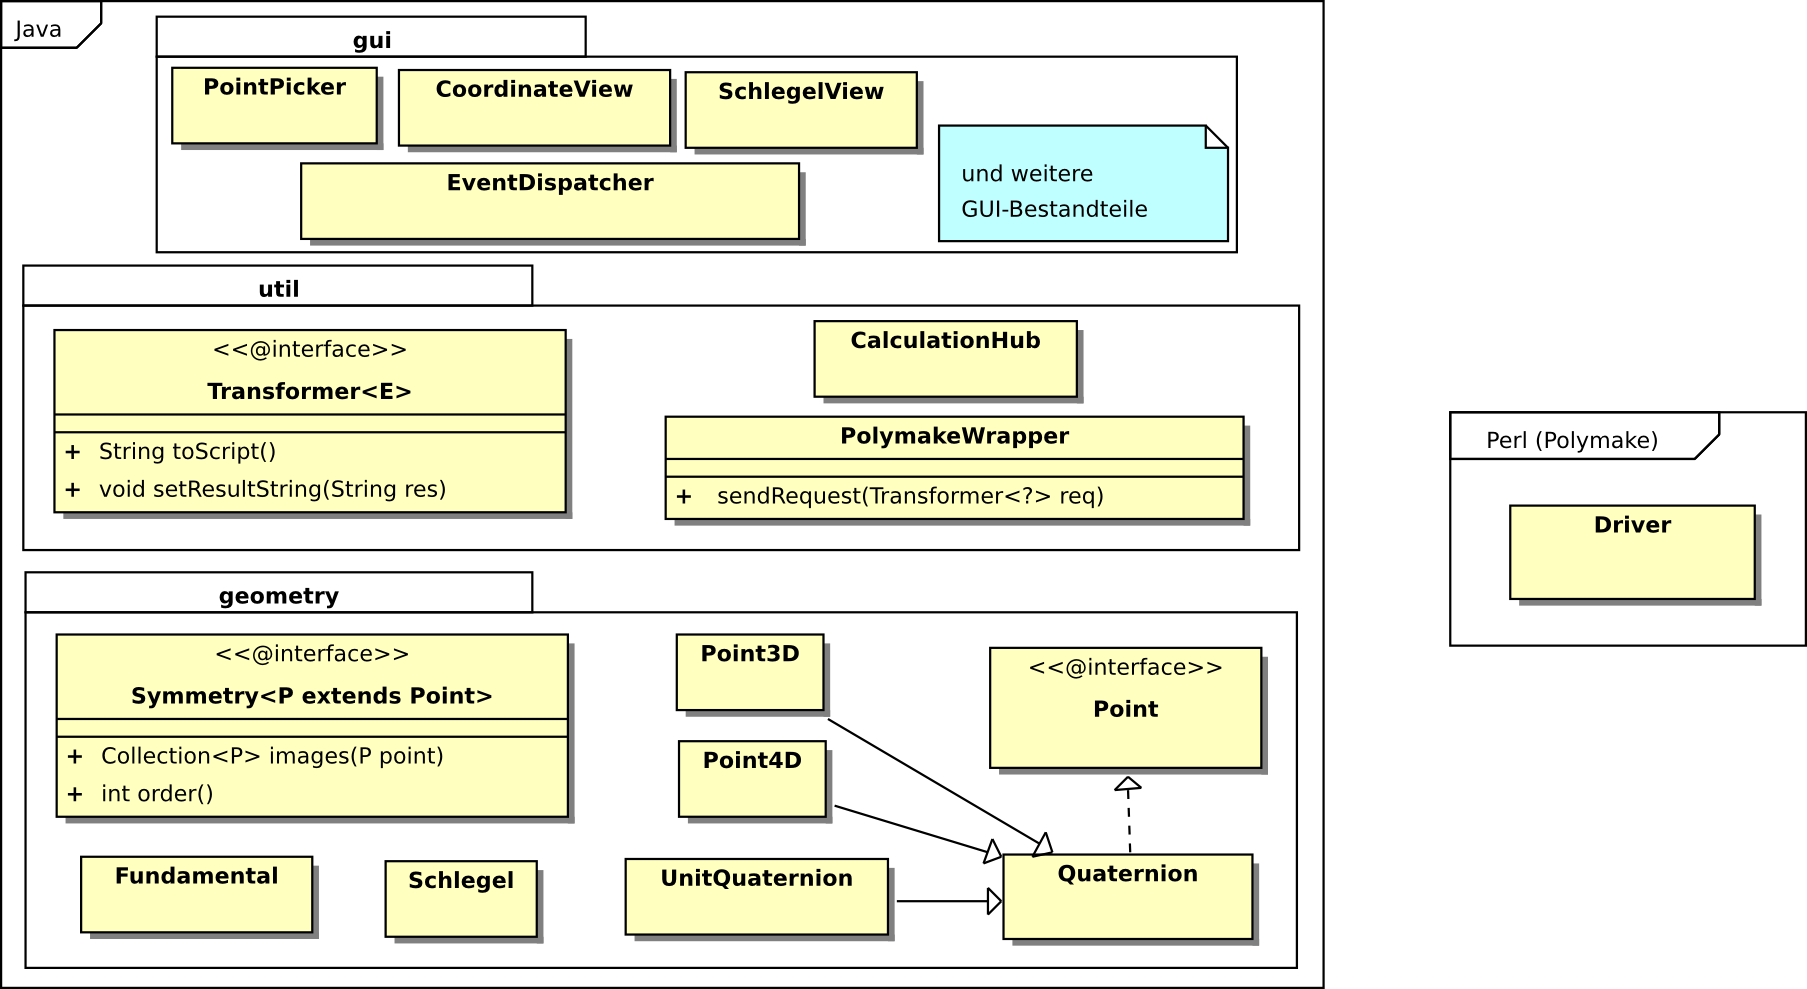
\includegraphics[width=0.85\textwidth]{img/architecture}
            \caption{Grobübersicht über die Architektur des Projekts\label{fig:architecture}}
        \end{figure}
    \begin{itemize}
        \item Pipeline-artiger Informationsfluss (siehe~\ref{ssec:flow})
        \item Lose Kopplung durch Eventsystem (siehe~\ref{ssec:event})
        \item Aufbereitung der Daten durch GUI (siehe~\ref{ssec:gui})
    \end{itemize}
    Grobidee skizzieren: Wir verwenden polymake als externen rechner und verwalten zustand/gui selbst. anzeige wird mit hilfe von jreality gemacht....integriert, blabla.

    \subsubsection{Verwendete Softwarehilfsmittel}
       \begin{description}
           \item jReality~\cite{jreality} jeweils 1-2 saetze was /wofür das ist
           \item [Polymake]
           	~\cite{polymake} ist ein Werkzeug um Berechnungen mit konvexen Polytopen (z.B. das Berechnen von konvexen Hüllen) auszuführen. Es wird entweder als Kommandozeilenanwendung oder online benutzt.
           \item maven~\cite{maven} jeweils 1-2 saetze was /wofür das ist
           \item [JUnit]
            ~\cite{jUnit} ist ein Framework zum Testen von Java-Anwendungen mittels Unit-Tests. Mit den Tests kann nach jeder Änderung oder Neuerung automatisiert getestet werden, ob Methoden fehlerfrei funktionieren und das gewünschte Resultat liefern.
        \end{description}

    \subsubsection{Informationsfluss\label{ssec:flow}}
        \begin{figure}[tbh]
            \centering
            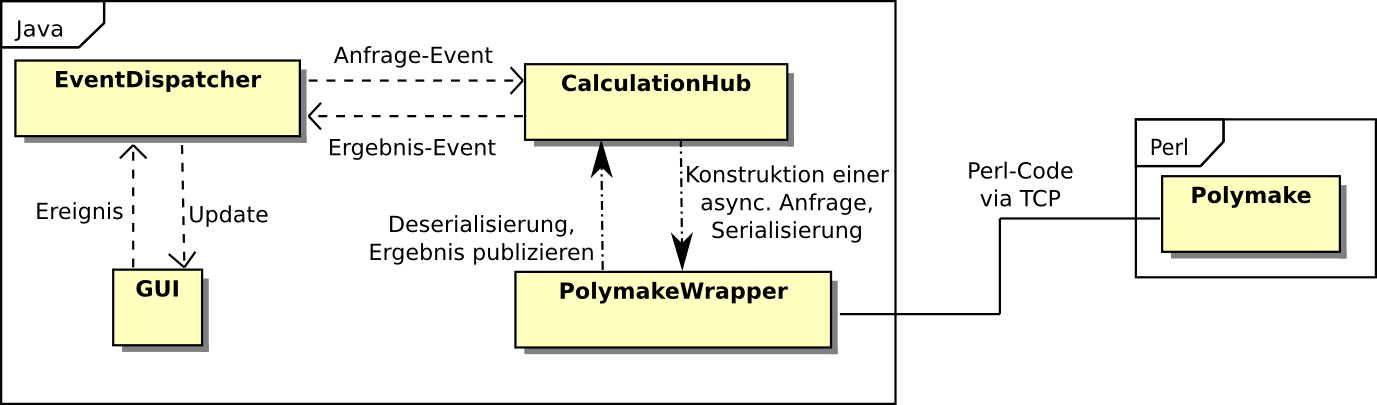
\includegraphics[width=0.85\textwidth]{img/flow}
            \caption{Informationsfluss zwischen den Komponenten
                      {\scriptsize(gestrichelt: sync. Methodenaufruf, punkt-strich: async. Methodenaufruf, durchgezogen: TCP-Nachricht}}
        \end{figure}

        yada yada 
    \subsubsection{Eventssystem\label{ssec:event}}
        \begin{figure}[bht]
            \centering
            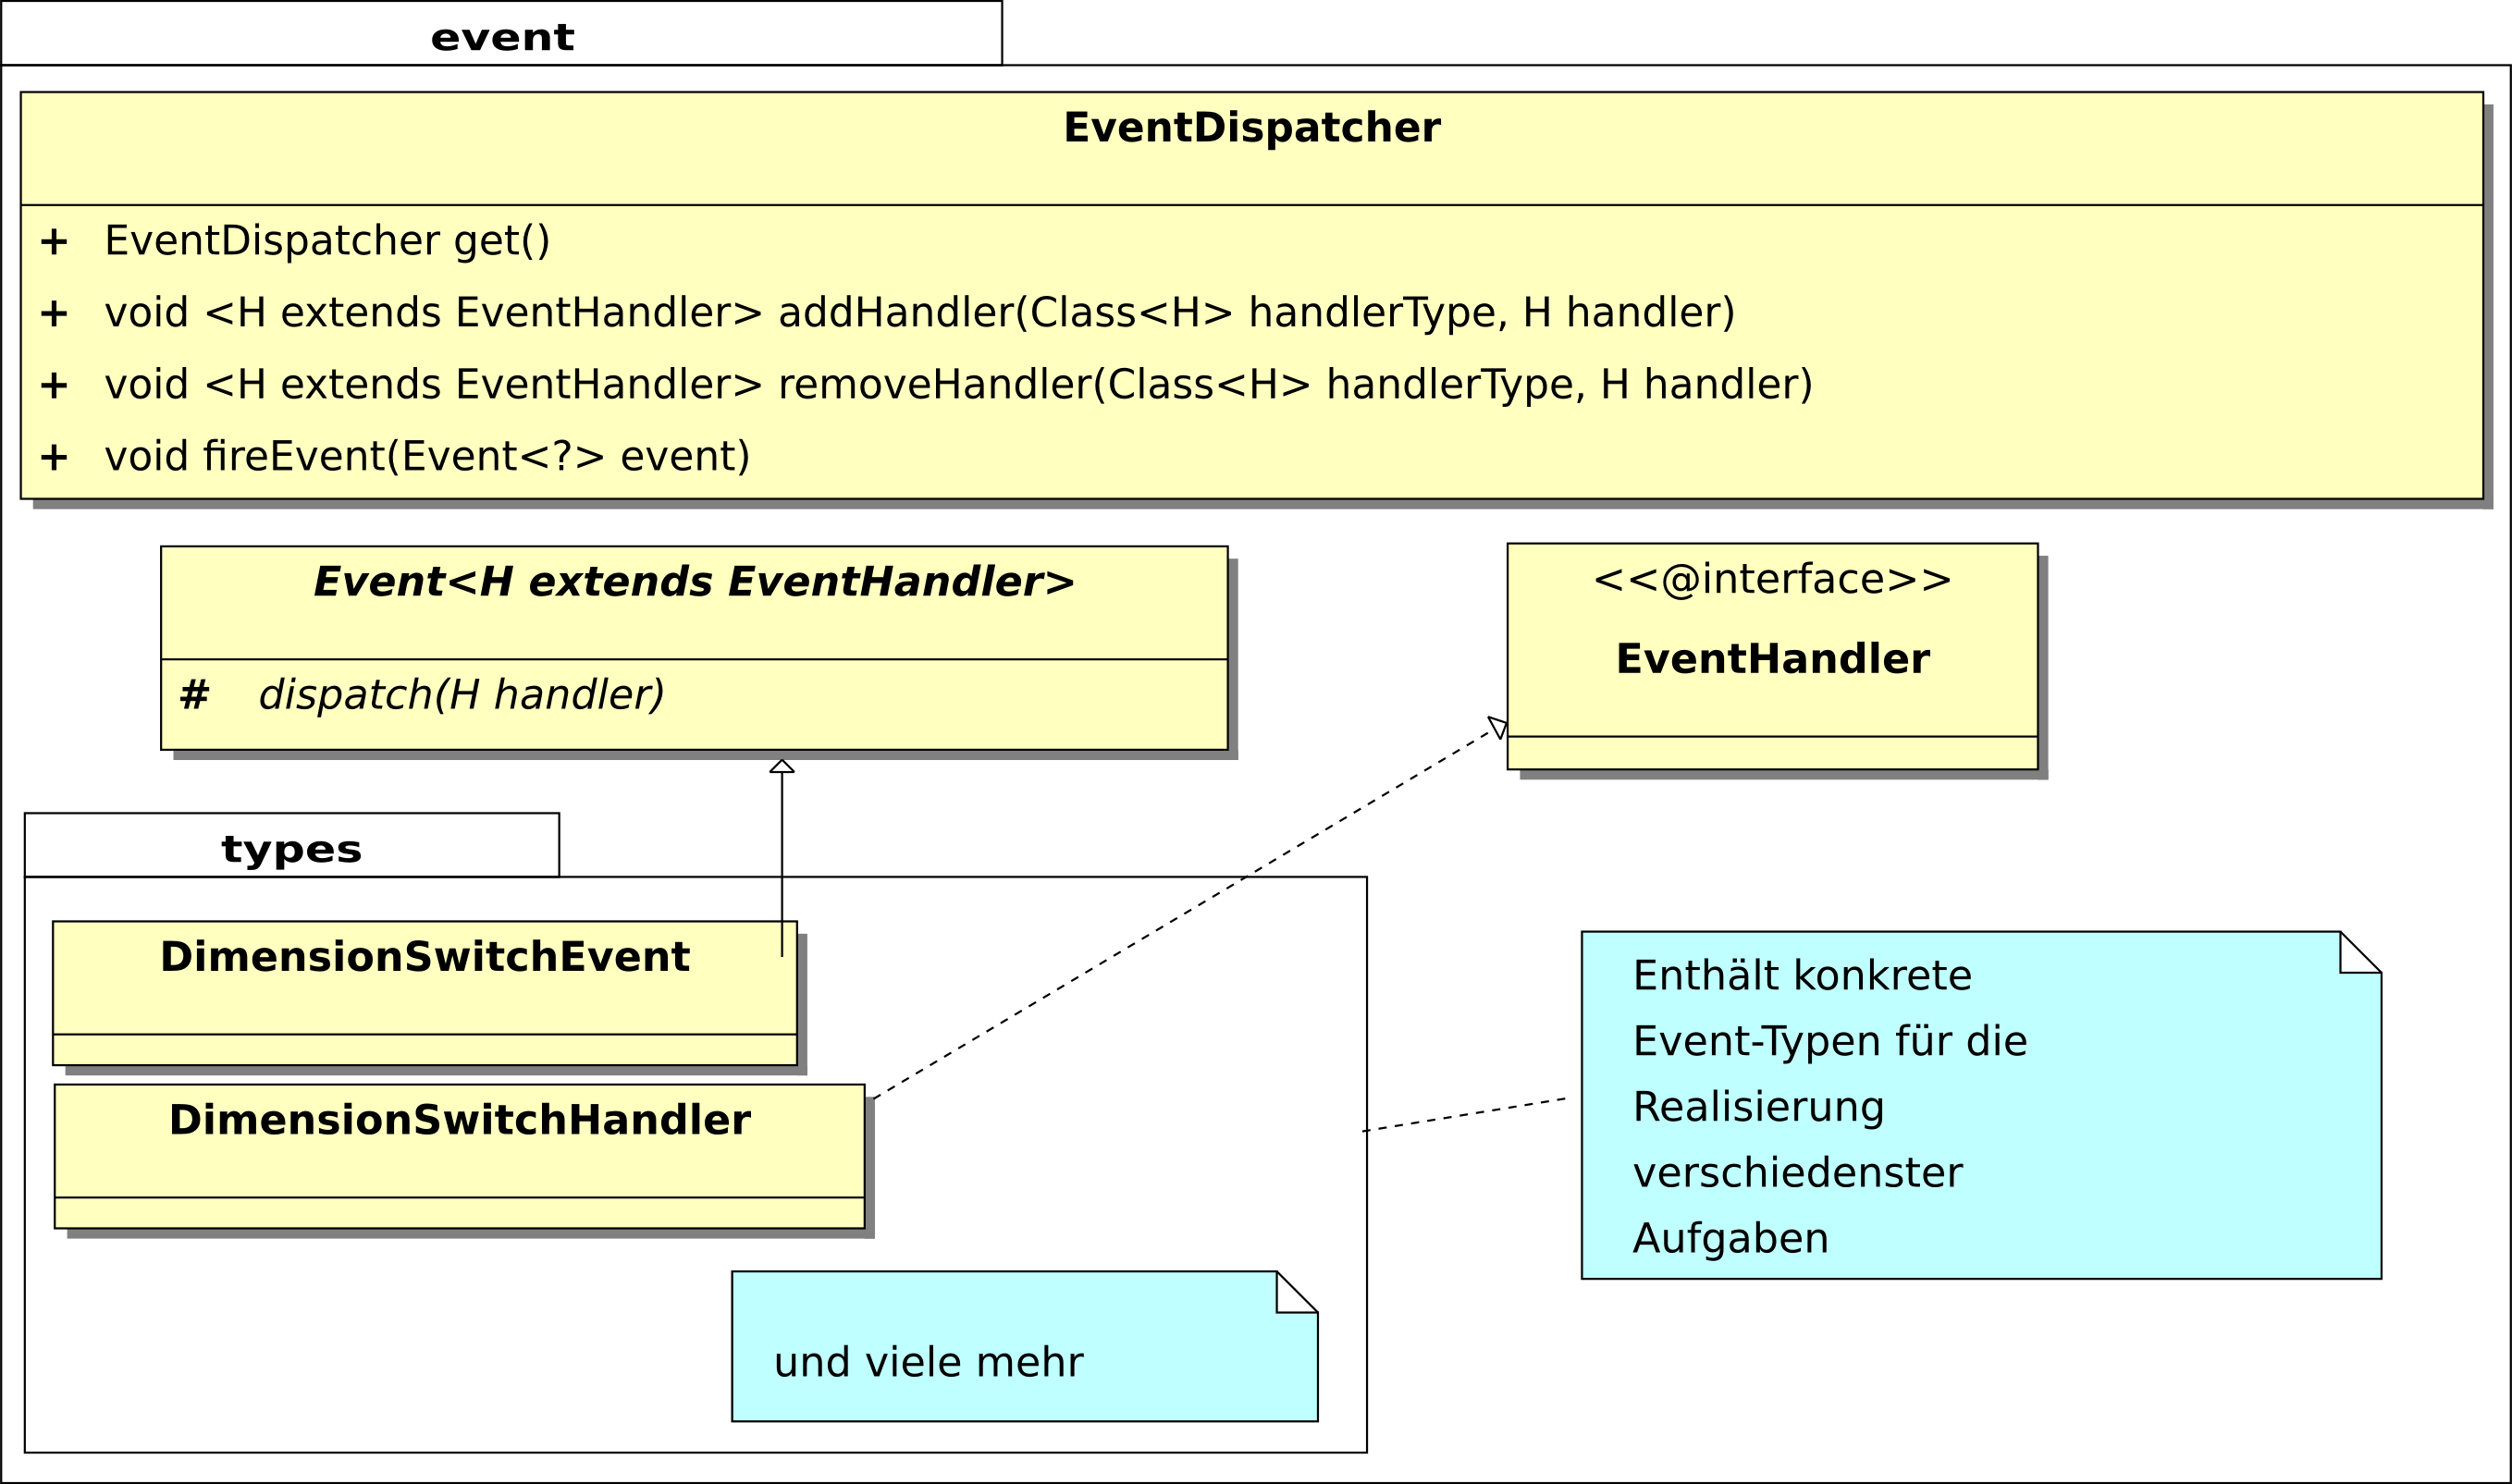
\includegraphics[width=0.8\textwidth]{img/event_classdiagram2}
            \caption{Klassendiagramm des Eventsystems}
        \end{figure}
        \subsubsection*{Events}
            Events sind konkrete Reaktionen auf bestimmte Ereignisse und enthalten je nach Ereignis entsprechende Kontextinformationen.
            Alle Typen von Events erben von der abstrakten Klasse \lstinline|Event<H extends EventHandler>| und stellen einen
            zugehörigen \lstinline|EventHandler|-Typen bereit.
            Komponenten, die auf ein bestimmtes Event reagieren sollen, realisieren das zum Event zugeordnete
            \lstinline|EventHandler|-Interface und implementieren damit eine Reaktionsmethode mit komponentenspezifischem
            Code.

            Eine zentrale Singleton-Instanz, der \lstinline|EventDispatcher|, koordiniert dann das Absenden und Empfangen von Events
            und verteilt die Ereignismeldungen an Interessenten.
            Hierfür muss jede an einem spezifischen Event interessierte Komponente sich als solche beim
            \lstinline|EventDispatcher| registrieren (\lstinline|addHandler(Class<H> eventType, H handler)|).
            Eine designierte Eventquelle hält ebenfalls einen Verweis, um mittels dessen
            \lstinline|fireEvent(Event<?> e)|-Methode im Zuge einer Reaktion ein Event abzufeuern.

      %  \subsubsection*{Eventimplementierung}
      %      Event-Typen werden durch Anlegen einer Event-Klasse und einer EventHandler-Klasse hinzugefügt.%
%
%            Das EventHandler-Template ist
%            
%            \begin{code}
%                import pointGroups.gui.event.EventHandler;
%
%                public interface ConcreteHandler
%                    extends EventHandler
%                {
%                    public void onConcreteEvent(final ConcreteEvent event);
%                }
%            \end{code}
%
%            Das Event-Typ-Template ist
%
%            \begin{code}            
%                import pointGroups.gui.event.Event;
%
%                public class ConcreteEvent
%                    extends Event<ConcreteHandler>
%                {
%                    public final static Class<ConcreteHandler> TYPE =
%                        ConcreteHandler.class;
%
%                    @Override
%                    public final Class<ConcreteHandler> getType() {
%                        return TYPE;
%                    }
%
%                    @Override
%                    protected void dispatch(final ConcreteHandler handler) {
%                        handler.onConcreteEvent(this);
%                    }
%                } 
%            \end{code}
%            
%            wobei Concrete durch konkrete Namen ersetzt werden kann.
            
        \subsubsection{GUI\label{ssec:gui}}
             MARCEL: ein bisschen erzählen, woher jreality kommt und warum wir es benutzen (in frame eingebettet etc). was es kann, wie wir es bisschen anpassen mussten.
                
\subsection{Implementierung von Berechnungen}
    \subsubsection{Symmetriebilder}
        ALEX SCHREIBT HIER KURZEN PSEUDOCODE    
    \subsubsection{Symmetriegruppen}
        OLLI SCHREIBT HIER ZU .... Symmetriegruppen (Berechnung mittels Generatoren, hart kodiert, Darstellung/Repräsentation)
    \subsubsection{Fundamentalbereich}
         In Abschnitt \ref{fundamentalbereich} wurde in Definition \ref{fundamentalbereich:voronoi} der Voronoi-Fundamentalbereich beschrieben. Zur Berechnung der Punktgruppen soll eine dieser Zellen ausgewählt und visualisiert werden.
         Zur einfacheren Darstellung eines Abschnitts der Sphäre $S^3$ berechnen wir zunächst die Projektion des Voronoi--Fundamentalbereichs auf eine $\mathbb{R}^3$ Ebene.
        \subsubsection*{Idee}
            Wir lassen zunächst die Symmetriegruppe auf ein ausgezeichnetes Element $x$ wirken.

            Als erstes Berechnen wir die Voronoi--Zelle für $x$ bezüglich des Orbits von $x$. Alle Punkte die innerhalb dieser Voronoi--Zelle liegen, sind Elemente von $S^3$. 
            Da die Gruppe symmetrisch ist, können wir nicht zwei Elemente aus dem selben Orbit haben. 
            Andernfalls müsste ein zweiter Punkt näher an einem anderen Element aus $G \rhd x$ liegen.
            Dabei ist es notwendig, dass sich der Punkt $x$ nicht auf einer Rotationsachse oder Spiegelebene befindet, da sonst die Voronoi--Zellen zu groß ausfallen.
            
            Anschließend projizieren wir diese Zelle auf eine Ebene, die tangential auf dem Kugelsegment liegt. Dazu wählen wir die Ebene $h \, : \, [t - x] \cdot x = 0$ in Normalendarstellung, da wir wissen, dass $x$ auf der Kugeloberfläche im Kreissegment liegt und $x$ auch ein Normalenvektor ist.
            
        \subsubsection*{Umsetzung}
         Eine Voronoi--Zelle von $x$ für eine Menge von Zentren $S$ ist definiert als 
         $$ VC(x) = \bigcap_{s \in S \setminus \{ x \}} h^+_{x,s}$$
         Wobei $h^+_{x,s}$ der Halbraum ist, der rechts von der Hyperebene liegt, die zu $x$ und $y$ in jedem Punkt den selben Abstand hat.\\
         
         In polymake kann die Voronoi--Zelle als Polytop über den Schnitt von den zugehörigen Halbräumen definiert werden. Dies geht über den Befehl

         \begin{code}
            new Polytope(INEQUALITIES=>\$hyperplanes)
         \end{code}

         Dabei ist \$hyperplanes eine Menge von Hyperebenen. Falls ein affines Polytop vorliegt, wie in unserem Fall in der Ebene $h$, die wie im letzten Abschnitt
         definiert ist, können wir auch dies mit in die Erzeugung mittels

         \begin{code}
            new Polytope(INEQUALITIES=>\$hyperplanes, EQUATIONS=>{h})
         \end{code}

         eingeben und haben so $VC(x)$ berechnet. \todo{Wieso wird die Ebene mit eingegeben?}
         
         Da die konkrete Berechnung über den Schnitt von allen Hyperebenen zu lange dauert, filtern wir die in frage kommenden Hyperebenen über die Nachbarn des Voronoi--Diagramms vor.
         Einen einfacheren Weg mittels polymake zur direkten Berechnung der Voronoi--Zelle konnten wir nicht auffinden. Daher dieses etwas umfangreichere Vorgehen.\\

         Das Polytop befindet sich nun in der Ebene. Für die Darstellung in $n-1$ Dimensionen berechnen wir nun eine geeignete Basis, so dass die Eckpunkte des Polytops durch $n-1$ Koordinaten darstellen werden können. 
         Der Punkt $x$ steht senkrecht auf der Ebene und ist damit für die Darstellung 
         unerheblich. Wir berechnen eine Orthonormalbasis für die Ebene mit $x$ als erstem Basisvektor. Nun können wir leicht eine Basiswechselmatrix angeben,
         da die Bilder der neuen in der alten Basis bekannt. Darüber hinaus ist diese Matrix orthogonal -- da die Spalten eine Orthogonalbasis waren, weshalb die zu diesem Basiswechsel inverse Matrix durch Transponieren einfach ermittelt werden kann.

         Wir haben nun also zwei Matrizen, um beide Darstellungen ineinander umzurechnen. In der neuen Basis können wir nun die erste Komponente weg lassen, da diese nach der Projektion auf null abgebildet wird. Daraus resultiert eine Darstellung in $n-1$ Dimensionen.
         Beim Zurückrechnen muss nur beachtet werden, dass sich die Punkte in einer affinen Ebene mit Stützvektor $x$ befinden.

        \subsubsection*{Berechnung}

         Die Definition von Hyperebenen in polymake hat die Darstellung
         $$
            h \, : \, [a_0, ..., a_n] \rightsquigarrow a_0 + a_1 x_1 + \cdots + a_n x_n = 0
         $$
         und entsprechend für Halbräume mit $\geq 0$.\\

         Die Halbräume für unser Polytop genügen der Gleichung
         $$
            t \cdot (x - s) \geq 0 \Leftrightarrow 0 + (x_1-s_1)\cdot t_1 + \cdots + (x_n -s_n)t_n \geq 0,
         $$
         wobei $x$ der gewählte Vektor war und $s \not x$ aus dem Orbit von $x$ stammt.

         Damit können wir alle Halbräume aus dem Orbit berechnen. Die affine Ebene genügt der Gleichung
         $$
            (t - x) \cdot x = 0 \Leftrightarrow - \left( \sum_{i=1}^n x_i^2 \right) + t_1 x_1 + \cdots t_n x_n = 0
         $$
         und kann auch leicht erstellt werden. Um das von uns gewünschte Polytop zu bekommen, benutzen wir das folgende polymake-Script

         \begin{code}
            my \$poly = new Polytope(INEQUALITIES=>\$hyperplanes, EQUATIONS=>\$affine);
            print \$poly->VERTICES;
            print \$poly->EDGES;
            print \$poly->FACETS;
         \end{code}

         Mit diesen Ergebnissen können wir nun die Basiswechselmatrizen berechnen und so die Punkte umrechnen. Das Objekt \emph{Fundamental} ist somit
         eine Sammlung dieser Eigenschaften.

         \begin{code}
            public interface Fundamental {
               public double[][] getVertices();
               
               public Edge<Integer,Integer>[] getEdges();

               public double[] revertPoint(double[] point);

               public boolean inFundamental(double[] point);
            }
         \end{code}
         
         Die ersten beiden Funktionen liefern entsprechend ihrer Namensgebung die Knoten und Kanten des Fundamentalbereichs. Die dritte Methode \emph{revertPoint} nimmt einen Punkt in $\mathbb{R}^{n-1}$ und
         hebt ihn auf die Oberfläche der $S^{n-1}$ zurück. Die letzte Methode überprüft, ob ein angegebener Punkt überhaupt in der Voronoi--Zelle liegt.
         Diese Methode wird bei der Anzeige benötigt, um bei der Punktauswahl keine Punkte außerhalb das Polytops auszuwählen.\\

         Das Ganze ist eine Schnittstelle, da wir als Fallback-case, falls die Berechnung das Fundamentalbereichs einmal fehl schlägt, immer noch 
         den Bereich $S^{n-2}$ benutzen können. Dies ist kein Fundamentalbereich, da wir alle Orbits mehrfach treffen. Allerdings werden wir, außer im Falle
         der Identität, jeden Orbit mindestens einmal treffen.
